% document formatting
\documentclass[10pt]{article}
\usepackage[utf8]{inputenc}
\usepackage[left=1in,right=1in,top=1in,bottom=1in]{geometry}
\usepackage[T1]{fontenc}
\usepackage{xcolor}

% math symbols, etc.
\usepackage{amsmath, amsfonts, amssymb, amsthm}
\usepackage{mathtools}

% lists
\usepackage{enumerate}
\usepackage{enumitem}

% images
\usepackage{graphicx} % for images
\usepackage{multirow}

% code blocks
\usepackage{minted, listings} 

% verbatim greek
\usepackage{alphabeta}

\graphicspath{{./assets/images}}

\newcommand{\solution}{\textbf{Solution:}} 
\newcommand{\example}{\textbf{Example: }}
\newcommand{\sinc}{\text{sinc}}
\newcommand{\rect}{\text{rect}}
\newcommand{\llra}{\Longleftrightarrow}
\newcommand{\fourier}{\mathcal{F}}
\newcommand{\laplace}{\mathcal{L}}
\newcommand{\absint}{\int_{-\infty}^\infty}
\newcommand{\dd}{\text{d}}

\title{EC ENGR 102 Week 9}

\author{Aidan Jan}
\date{\today}

\begin{document}
\maketitle

\section*{Partial Fractions, If Poles Could Be Repeated}
Our prior results were for non-repeated poles.  Sometimes, poles will be repeated.  Here,
\[F(s) = \frac{b(s)}{(s - \lambda_1)^k (s - \lambda_2) \cdots (s - \lambda_t)}\]
The poles $\lambda_i$ are distinct, but $\lambda_1$ has multiplicity $k$.\\\\
The partial fraction expansion for $F(s)$ will still have $n$ residues (where $n$ is the order of the polynomial $a(s)$ as before) but will involve higher powers of $(s - \lambda_1)$.  In particular, the expansion is:
\[F(s) = \frac{r_{1, k}}{(s - \lambda_1)^k} + \frac{r_{1, k - 1}}{(s - \lambda_1)^{k - 1}} + \cdots + \frac{r_{1, 1}}{(s - \lambda_1)} + \frac{r_2}{s - \lambda_2} + \cdots + \frac{r_l}{s - \lambda_l}\]
After achieving this expansion, we use the following inverse Laplace transform:
\[\laplace^{-1} \left[\frac{r}{(s - \lambda)^k}\right] = \frac{r}{(k - 1)!} t^{k - 1} e^{\lambda t}\]

\subsection*{Calculating the Residuals for Repeated Poles}
\begin{itemize}
    \item To calculate the residuals, we can use Method 1 as before.
\end{itemize}
We can also extend Method 2.  To get $r_{i, k}$, where $k$ is the multiplicity of the pole, we multiply both sides by $(s - \lambda_i)^k$ and evaluate at $s = \lambda_i$.  Hence,
\[r_{i, k} = F(s)(s - \lambda_i)^k\bigg|_{s = \lambda_i}\]
To get the other residues, $r_{i, k - j}$, we differentiate with respect to $s, j$ times, leading to the formula:
\[\frac{1}{j!} \frac{\dd^j}{\dd s^j}(F(s)(s - \lambda_i)^k) \bigg|_{s = \lambda_i} = r_{i. k - j}\]
To get an intuition for this, let's do an example.

\subsubsection*{Repeated Poles Example}
Let's find the partial fraction expansion of
\[\frac{1}{s^2(s + 1)} = \frac{r_{1, 2}}{s^2} + \frac{r_{1, 1}}{s} + \frac{r_2}{s + 1}\]
Using the cover-up method (Method 2):
\begin{itemize}
    \item $r_2$: $\frac{1}{s^2}\bigg|_{s = -1} = 1$
    \item $r_{1, 2}$: $\frac{s^2}{s^2(s+1)} = r_{1, 2} + r_{1, 1} \cdot s + \frac{r_2 \cdot s^2}{s + 1}$\\
    We then set $s = 0 \Rightarrow r_{1, 2} = \frac{1}{s + 1}\bigg|_{s = 0} = 1$
    \item To solve for $r_{1, 1}$, we first start with the same equation as for $r_{1, 2}$
    \begin{align*}
        \frac{s^2}{s^2(s+1)} &= r_{1, 2} + r_{1, 1} \cdot s + \frac{r_2 \cdot s^2}{s + 1}\\
        \intertext{We then take the derivative of both sides.}
        r_{1, 1}:\: \frac{\dd}{\dd s} \frac{1}{s + 1} &= \frac{\dd}{\dd s} \left[r_{1, 2} + r_{1, 1} \cdot s + \frac{r_2 \cdot s^2}{s + 1}\right]\\
        -\frac{1}{(s + 1)^2} &= r_{1, 1} + \frac{\dd}{\dd s} \left[\frac{r_2 s^2}{s + 1}\right]
        \intertext{Now we set $s = 0$.  (We didn't have to take the derivative of the $r_2$ term since it cancels out anyways.)}
        r_{1, 1} &= -\frac{1}{(0 + 1)^2} = -1
    \end{align*}
\end{itemize}

\subsection*{Quadratic Factors}
Let's consider the example we did earlier:
\[V(s) = \frac{s^2}{s^3 - 1} = \frac{s^2}{(s - 1)(s^2 + s + 1)}\]
The partial fraction expansion is:
\[\frac{s^2}{(s - 1)(s^2 + s + 1)} = \frac{r_1}{s - 1} + \frac{r_2 s + r_3}{s^2 + s + 1}\]
First, we can solve for $r_1$ using Method 2.
\[r_1 = \frac{s^2}{s^2 + s + 1}\bigg|_{s = 1} = \frac{1}{3}\]
Hence, we now have that:
\[\frac{s^2}{(s - 1)(s^2 + s + 1)} = \frac{1/3}{s - 1} + \frac{r_2 s + r_3}{s^2 + s + 1}\]
Solve for $r_3$ by setting $s = 0$ to eliminate $r_2$ yields:
\[0 = \frac{1/3}{-1} + r_3\]
Therefore, $r_3 = \frac{1}{3}$.\\\\
Finally, we can solve for $r_2$.
\[\frac{s^2}{(s - 1)(s^2 + s + 1)} = \frac{1/3}{s - 1} + \frac{r_2 s + 1/3}{s^2 + s + 1}\]
Let's set $s = -1$ (since setting $s = 1$ would make one term undefined).
\[\frac{1}{-2 \cdot 1} = -\frac{1}{6} + \frac{-r_2 + 1/3}{1}\]
Solving for $r_2$ gives $r_2 = 2/3$.\\\\
Now, we have to factor the term
\[\frac{\frac{2}{3} s + \frac{1}{3}}{s^2 + s + 1}\]
into an expression where we can take the inverse Laplace transform.  We do this by completing the square.\\\\
Referring the the Common Laplace Transform table, we see that
\[\laplace[e^{-at}\cos(\omega t)] = \frac{(s + a)}{(s + a)^2 + \omega^2}\]
Therefore, we can rewrite the numerator as
\[\frac{2}{3} s + \frac{1}{3} = \left(\frac{2}{3}\right)\left(s + \frac{1}{2}\right)\]
E.g., $a = \frac{1}{2}$.  Now, we have to get the denominator into the form
\[s^2 + s + 1 = \left(s + \frac{1}{2}\right)^2 + \omega^2\]
By completing the square, we can solve that $\omega^2 = \frac{3}{4}$, and therefore, $\omega = \frac{\sqrt{3}}{{2}}$.\\\\
Now, we have:
\[\frac{\frac{2}{3}s + \frac{1}{3}}{s^2 + s + 1} = \frac{\frac{1}{3}}{s - 1} + \left(\frac{2}{3}\right)\frac{s + \frac{1}{2}}{(s + \frac{1}{2})^2 + (\frac{\sqrt{3}}{2})^2}\]
By look up table, the inverse Laplace transform is:
\[v(t) = \frac{1}{3}e^t + \frac{2}{3}e^{-t/2} \cos\left(\frac{\sqrt{3}}{2}t\right)\]
\subsection*{Which Method to Use? (Informal)}
\begin{itemize}
    \item Use Method 2.
    \item Sometimes, you can use Method 3 to minimize algebra.  If it does not give an obviously simple solution, avoid it.
    \item Never use Method 1 since the algebra can get involved.
    \item In case of complex roots, the first approach of finding complex roots is more straightforward (using Euler's identities).  However, complex arithmetic is more prone to errors.
    \item Quadratic factors may be straightforward, while the residues are easy to calculate.  However, it requires the extra step of completing the square to get the final answer.
\end{itemize}
\pagebreak
\section*{Nonproper Rational Functions}
The partial fraction expansion that we've talked about earlier is for a \textit{strictly proper} $F(s)$, with $m < n$.
\[F(s) = \frac{b(s)}{a(s)} = \frac{b_0 + b_1 s + \cdots + b_m s^m}{a_0 + a_1 s + \cdots + a_n s^n}\]
There may be $F(s)$ for which this is not true and we want to find the Laplace transform of.  To do so, we perform:
\begin{align*}
    F(s) &= \frac{b(s)}{a(s)}\\
    &= c(s) + \frac{d(s)}{a(s)}
\end{align*}
where 
\[c(s) = c_0 + c_1 s + \cdots + c_{m-n}s^{m-n}\]
and 
\[d(s) = d_0 + \cdots d_k s^k\]
where $k < n$.  By intuition, we are basically converting the nonproper rational function into a polynomial plus a proper rational function.  (In this case, $\frac{d(s)}{a(s)}$ is proper.)\\\\
In this manner, we have split $F(s)$ into a component $c(s)$ and then a strictly proper component $d(s) . a(s)$.  For notation, we denote $\delta^k$ to be the $k$-th derivative of the $\delta$ function.  The inverse Laplace transform of $F(s)$ is therefore:
\[\laplace^{-1}[F(s)] = c_0 \delta(t) + c_1 \delta^{(1)}(t) + \cdots + c_{m - n}\delta^{(m - n)}(t) + \laplace^{-1}\left[\frac{d(s)}{a(s)}\right]\]
where we use partial fractions to represent $d(s) / a(s)$.\\\\
In this class, we haven't talked about what derivatives of delta functions mean.  You will not be responsible for them, and if we ever give a nonproper rational function, we will have $m = n$, so at most there is a $\delta$ function in the inverse Laplace transform.  We have presented this for the sake of "completeness".

\subsection*{Nonproper Rational Function Example}
Let
\begin{align*}
    F(s) &= frac{5s + 3}{s + 1}\\
    \intertext{In this case, we just do long division.}
    &= \frac{5s}{s + 1} + \frac{3}{s + 1}\\
    &= \frac{5(s + 1)}{s + 1} - \frac{5}{s + 1} + \frac{3}{s + 1}\\
    &= 5 - \frac{2}{s + 1}
\end{align*}
Now, we can take the inverse Laplace transform:
\[f(t) = 5 \cdot \delta(t) - 2e^{-t},\hspace{1cm} \text{ for $t \geq 0$}\]

\subsection*{Another Example}
\[F(s) = \frac{s^4 + s^3 - 2s^2 + 1}{s^3 + 2s^2 + s} = c(s) + \frac{d(s)}{a(s)}\]
To solve this, we do long division.  (Or synthetic Division)
\begin{center}
    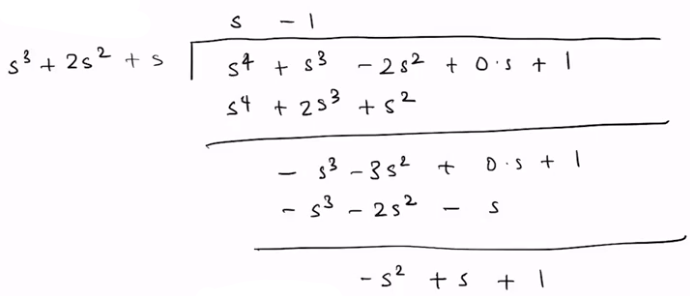
\includegraphics[scale=0.7]{W10_1.png}
\end{center}
\begin{align*}
    F(s) &= s - 1 + \frac{-s^2 + s + 1}{s^3 + 2s^2 + s}
\end{align*}
Now, we have
\begin{align*}
    \frac{d(s)}{a(s)} &= \frac{-s^2 + s + 1}{s^3 + 2s^2 + s} = \frac{-s^2 + s + 1}{s(s^2 + 2s + 1)} = \frac{-s^2 + s + 1}{s \cdot (s + 1)^2}\\
    &= \frac{r_1}{s} + \frac{r_{2, 1}}{s + 1} + \frac{r_{2, 2}}{(s + 1)^2}
\end{align*}
\begin{itemize}
    \item $r_1$: $\frac{-s^2 + s + 1}{(s + 1)^2} \bigg|_{s = 0} = \frac{0 + 0 + 1}{1^2} = 1$
    \item $r_{2, 2}$: $\frac{-s^2 + s + 1}{s}\bigg|_{s = -1} = \frac{-1 - 1 + 1}{-1} = 1$
    \item $r_{2, 1}$: $\frac{-s^2 + s + 1}{s(s + 1)^2} = \frac{1}{s} + \frac{r_{2, 1}}{s + 1} + \frac{1}{(s + 1)^2}$\\\\
    Setting $s = 1$ gives:
    \begin{align*}
        \frac{-1 + 1 + 1}{1 (4)} &= 1 + \frac{r_{2, 1}}{2} + \frac{1}{4}\\
        \Rightarrow r_{2, 1} &= -2
    \end{align*}
\end{itemize}
\section*{$\uparrow$ FINAL EXAM COVERS UP TO HERE! $\uparrow$}
\subsection*{Applications of the Laplace Transform}
This lecture is about applications of the Laplace transform.  Topics include:
\begin{itemize}
    \item Linear constant coefficient ordinary differential equations (LCCODEs).
    \item Poles and zeros: intuition
    \item Filters and bode plots
    \item Feedback
\end{itemize}
Several examples in these lecture notes, including ODE examples, are thanks to Prof. John Pauly.
\subsection*{LCCODEs}
The Laplace transform allows us to straightforwardly solve linear differential equations that have:
\begin{itemize}
    \item Constant coefficients.
    \item Initial conditions
    \item Input signals
\end{itemize}
The procedure to solve for such a linear constant coefficient differential equation (LCCODE) is to:
\begin{enumerate}
    \item Use the Laplace transform to convert the differential equation, initial conditions, and input signals into an algebraic equation.
    \item Solve for the Laplace transform of the output.
    \item Invert the Laplace transform of the output.
\end{enumerate}
Importantly, the Laplace transform enables us to separate out the contriobution of the output fropm the \textit{initial conditions} of the ODE versus the \textit{inputs} to the system.
\subsubsection*{LCCODE Example}
Consider the LCCODE
\[y''(t) + 5y'(t) + 6y(t) = x'(t) + x(t)\]
Initial conditions: $y(0) = 2$, $y'(0) = 1$.  The input is $x(t) = e^{-4t} u(t)$.\\\\
Contribution of initial conditions is the solution $y(t)$ when $x(t) = 0$.  "Zero Input Response".  Left hand side of the LCCODE.\\\\
Contribution due to the input, when initial conditions is zero, "Zero State Response".  Right hand side of the equation affects the LCCODE.\\\\
\textbf{Contribution from the initial condition:} If we want the contribution from the initial condition, then we treat $x'(t) + x(t) = 0$.  This is the same as solving for the Laplace transform of the left hand side of the differential equation (which we would have had to do anyways).  So, taking the Laplace transform of the left hand side, we have:
\begin{align*}
    s^2 Y(s) - sy(0) &- y'(0) + 5(sY(s) - y(0)) + 6Y(s)\\
    &= Y(s)(s^2 + 5s + 6) - 2s - 1 - 10\\
    &= Y(s)(s^2 + 5s + 6) - (2s + 11) = 0
\end{align*}
With this equation, we can now assign it to equal zero (e.g., Zero input and zero state), and solve for $Y(s)$.
\begin{center}
Zero input response: $Y(s) = \frac{2s + 11}{s^2 + 5s + 6}$
\end{center}
\textbf{Contribution from the input:} To find the contribution from the input, we take the Laplace transform of the right hand side, which is:
\begin{align*}
    sX(s) - x(0) + X(s) &= X(s)(s + 1)\\
    &= \frac{s + 1}{s + 4}
\end{align*}
since $e^{-4t} u(t) \llra (s + 4)^{-1} = \frac{1}{s + 4}$.\\\\
This gives that the Laplace transform of the LCCODE is:
\[Y(s)(s^2 + 5s + 6) - (2s + 11) = \frac{s + 1}{s + 4}\]
Hence,
\[Y(s) = \frac{2s + 11}{s^2 + 5s + 6} + \frac{s + 1}{(s + 4)(s^2 + 5s + 6)}\]
Now, the terms
\begin{itemize}
    \item $\frac{2s + 11}{s^2 + 5s + 6}$ is the contribution to the output due to the initial conditions (since this is the Laplace transform when the inputs are zero).
    \item $\frac{s + 1}{(s + 4)(s^2 + 5s + 6)}$ is therefore the contribution to the output due to the input.
\end{itemize}
We're going to solve this in two ways.
\begin{enumerate}
    \item First, we'll solve the entire LCCODE giving the total output response due to both initial conditions and inputs.
    \item Second, we'll solve for $y(t)$ as a function of the contributions from the initial condition (called \textbf{zero input} solution) and from the input (called \textbf{zero state} solution).
\end{enumerate}
We'll confirm these give identical solutions.\\\\
First, solving for the total output response, ignoring what is from initial condition and what is from input.  So we'll first combine terms.
\begin{align*}
    Y(S) &= \frac{2s + 11}{s^2 + 5s + 6} + \frac{s + 1}{(s + 4)(s^2 + 5s + 6)}\\
    &= \frac{r_1}{s + 2} + \frac{r_2}{s + 3} + \frac{r_3}{s + 4}
\end{align*}
If we solve for the roots, we get $r_1 = 13/2$, $r_2 = -3$, $r_3 = -3/2$.
\[y(t) = \frac{13}{2}e^{-2t} - 3e^{-3t} - \frac{3}{2} e^{-4t}, \hspace{1cm}\text{ for $t \geq 0$}\]
\textbf{Zero input:} To solve the zero input term, $y_{zi}(t)$, we take the inverse Laplace transform of
\[\frac{2s + 11}{(s + 2)(s + 3)} = \frac{r_1}{s + 2} + \frac{r_2}{s + 3} = \frac{7}{s + 2} - \frac{5}{s + 3}\]
giving
\[y_{zi}(t) = [7e^{-2t} - 5e^{-3t}]u(t)\]
This is the zero input response, i.e., if $x(t) = 0$, this is what the output of the ODE would be.\\\\
\textbf{Zero state:} To solve for the zero state (i.e., no initial condition) term, $y_{zs}(t)$, we take the inverse Laplace transform of
\begin{align*}
    \frac{s + 1}{(s + 2)(s + 3)(s + 4)} &= \frac{r_1}{s + 2} + \frac{r_2}{s + 3} + \frac{r_3}{s + 4}\\    
    &= -\frac{1/2}{s + 2} + \frac{2}{s + 3} + \frac{3/2}{s + 4}
\end{align*}
which gives that
\[y_{zs}(t) = \left[-\frac{1}{2} e^{-2t} + 2e^{-3t} - \frac{3}{2} e^{-4t}\right]u(t)\]
Hence, the total solution is
\begin{align*}
    y(t) &= y_{zi}(t) + y_{zs}(t)\\
    &= [7e^{-2t} - 5e^{-3t}]u(t) + \left[-\frac{1}{2} e^{-2t} + 2e^{-3t} - \frac{3}{2} e^{-4t}\right]u(t)
\end{align*}
You can confirm that the sum of these terms is equal to the total solution we earlier derived, i.e., 
\[y(t) = \left[\frac{13}{2}e^{-2t} - 3e^{-3t} - \frac{3}{2}e^{-4t}\right]u(t)\]


\end{document}